% !TEX root = main.tex

\chapter{Motivation}
\label{ch:motivation}
\noindent

\newcommand{\officialp}{official prose}
\newcommand{\spectecp}{SpecTec prose}

\red{TODO: explanation of the terms \officialp{} and \spectecp{}} \\
\red{TODO: remove redundant part in the fig} \\
\red{TODO: explanation of context(frame/label): in the background? or here?} \\
\red{TODO: the notion of meta-level interpreter in background} \\
\red{TODO: try finding better terminology rather than "model"} \\


\section{Control flow in official prose}

% control flow structure in official prose
It might be easy to understand how the \officialp{} explains the control flow
of WebAssembly, if we assume that a WebAssembly code is loaded on a memory and
a pc points to the instruction to execute.
To describe control flow, it uses a structure named \textit{block} which
consitutes of a instruction sequence.
When executing the instructions in the block, pc can be changed to the starting
point of the block or the end of the block.


% an example of Wasm control flow in official prose
\textbf{Example 1}
\begin{verbatim}
  // infinite loop
  (loop (result i32) (i32.const 42) (br 0) (unreachable) end) (unreachable)
\end{verbatim}

Example 1 is a WebAssembly code example that has \texttt{loop} and
\texttt{unreachable}
Here, result type of the \texttt{loop} is \texttt{i32} and the \texttt{loop}
has a block of three instructions: \texttt{i32.const}, \texttt{br}, and
\texttt{unreachable}.
\cref{fig:loop} is the \officialp{} of the \texttt{loop} instruction.
It says that the continuation is the start of the loop, the information is
stored in a label, and it \textit{enters} the block with the label.
The term \textit{enter} means that it pushes the label in the stack and makes
pc points to the first instruction in the block.
The \texttt{i32.const} instruction is executed first, which just pushes the
\texttt{i32} value \texttt{42} in the stack.
Then, The \texttt{br} instruction is executed.
\cref{fig:br} is the \officialp{} of the \texttt{br} instruction.
It pops the label from the stack, and makes pc points to the continuation of
the label, which is the start of the loop instruction.
As a result, the code example above is a infinite loop pushing \texttt{42}
forever without executing \texttt{unreachable} instructions.

\begin{figure}[h!]
    \centerline{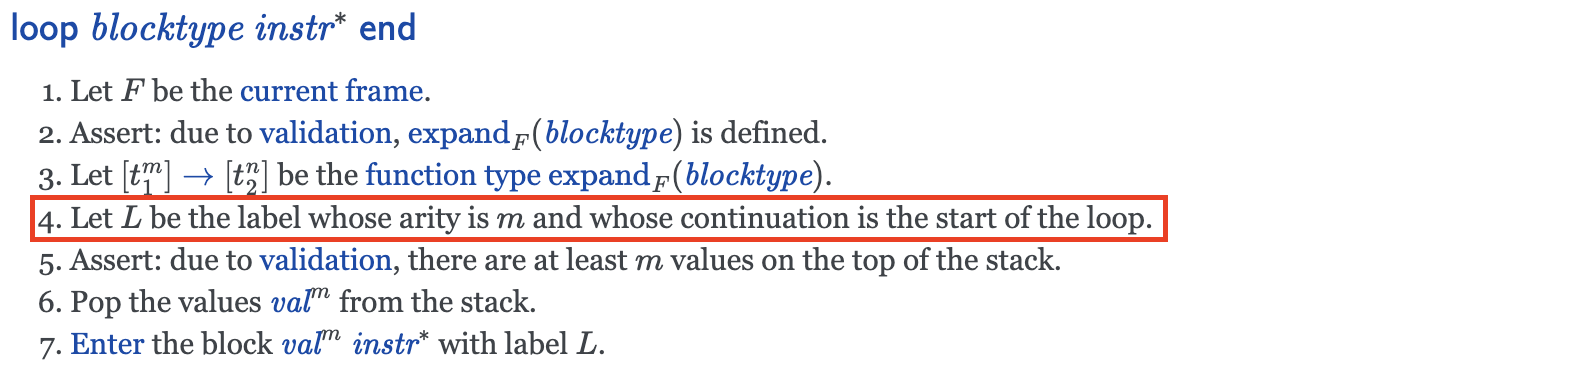
\includegraphics[width=15cm]{fig/loop}}
    \caption[Enter the caption title here]{\texttt{loop} instruction} \label{fig:loop}
    \centerline{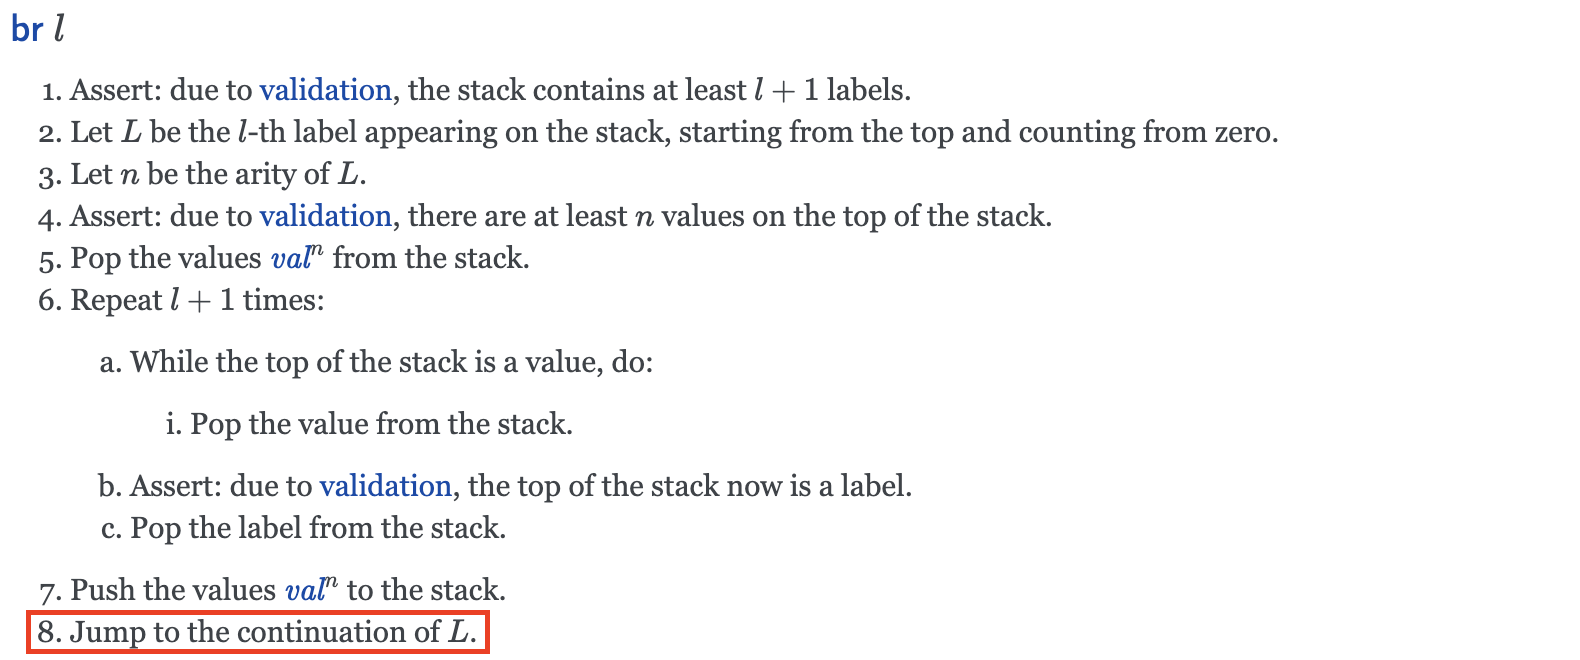
\includegraphics[width=15cm]{fig/br}}
    \caption[Enter the caption title here]{\texttt{br} instruction} \label{fig:br}
\end{figure}


% exiting label in official prose
There is also a special form of a behavior related to the block: an
\textit{exiting label}.
\cref{fig:exiting-label} is the \officialp{} of the \textit{exiting label}.
It is special because this behavior is performed without an explicit
WebAssembly instruction.
Rather, the behavior is performed when \textbf{the end of a block is reached}
without control instructions or runtime error.
The behavior is that the label is popped from the stack, and the pc changes to
the point after the end of the block.

\begin{figure}[h!]
    \centerline{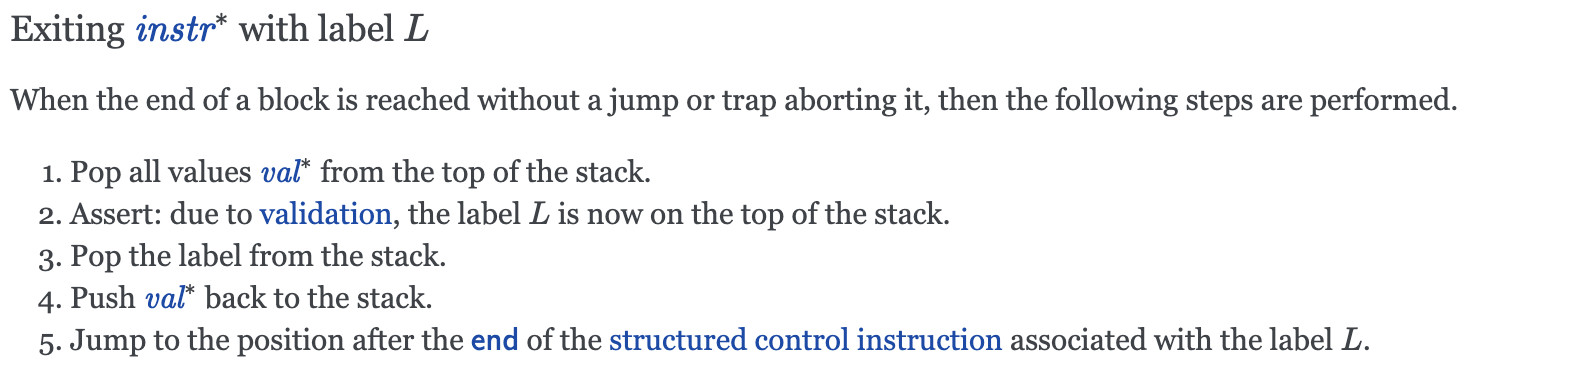
\includegraphics[width=15cm]{fig/exiting}}
    \caption[Enter the caption title here]{exiting label} \label{fig:exiting-label}
\end{figure}


% an example of exiting label in official prose
\textbf{Example 2}
\begin{verbatim}
  // exiting label
  (loop (result i32) (i32.const 42) end) (f64.const 3.14)
\end{verbatim}

Example 2 is a WebAssembly code example that has \texttt{loop} whose block is
only \texttt{i32.const}, and \texttt{f32.const}
When the \texttt{loop} instruction is executed, a label is pushed in the stack,
and it enters the block.
After \texttt{i32.const} is executed, the end of the block is reached.
As a result, exiting label occurs so that the label is popped from the stack,
pc changes to the point after the end of block: \texttt{f64.const}.
As a result, after executing the code, the value 42 and 3.14 pushed to the
stack.


% control flow structure with function call in official prose
Similar to the control flow using the block and the label, there is a function
call with a frame.
\cref{fig:invoke} is the \officialp{} of the function invocation which takes
place by a \texttt{call} instruction.
A frame is pushed to the stack and enters the block of the function body with a
label.
There is also a special behavior named returning from a function.
\cref{fig:returning} is the \officialp{} of the returning from a function.
When end of function is reached without without control instructions or runtime
error, The frame is popped from the stack, and the pc points to the next
instruction of the caller instruction.

\begin{figure}[h!]
    \centerline{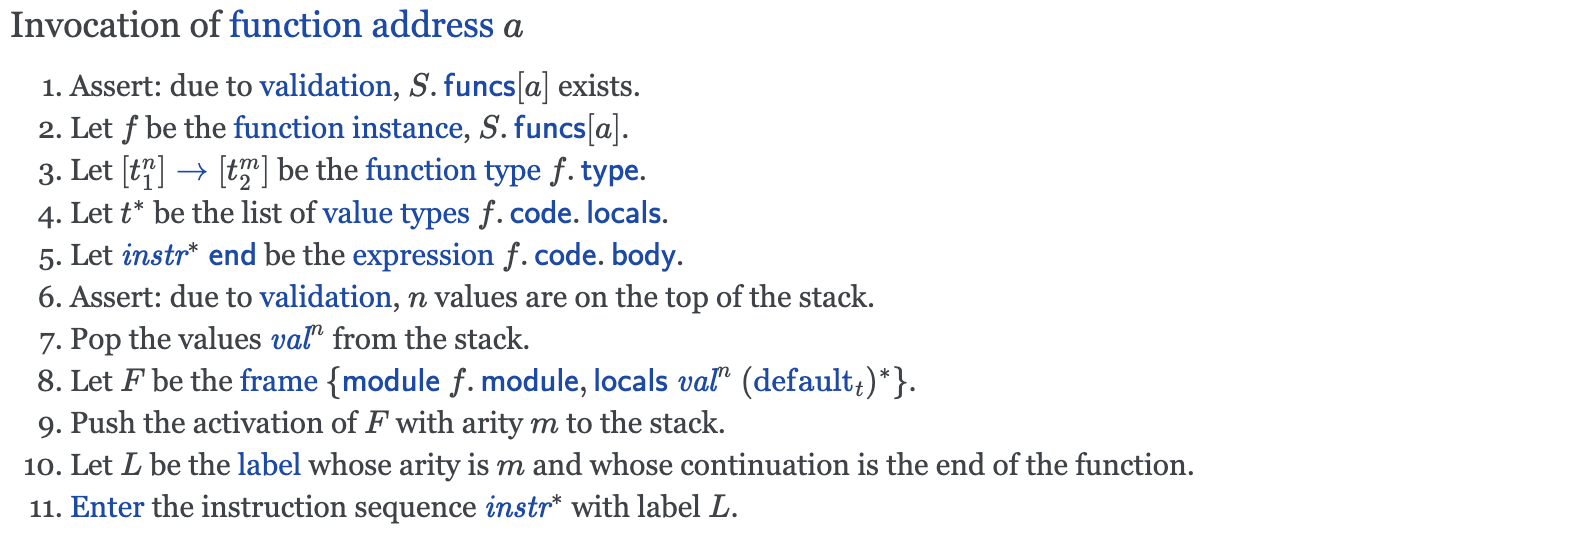
\includegraphics[width=15cm]{fig/invoke}}
    \caption[Enter the caption title here]{function invocation} \label{fig:invoke}
    \centerline{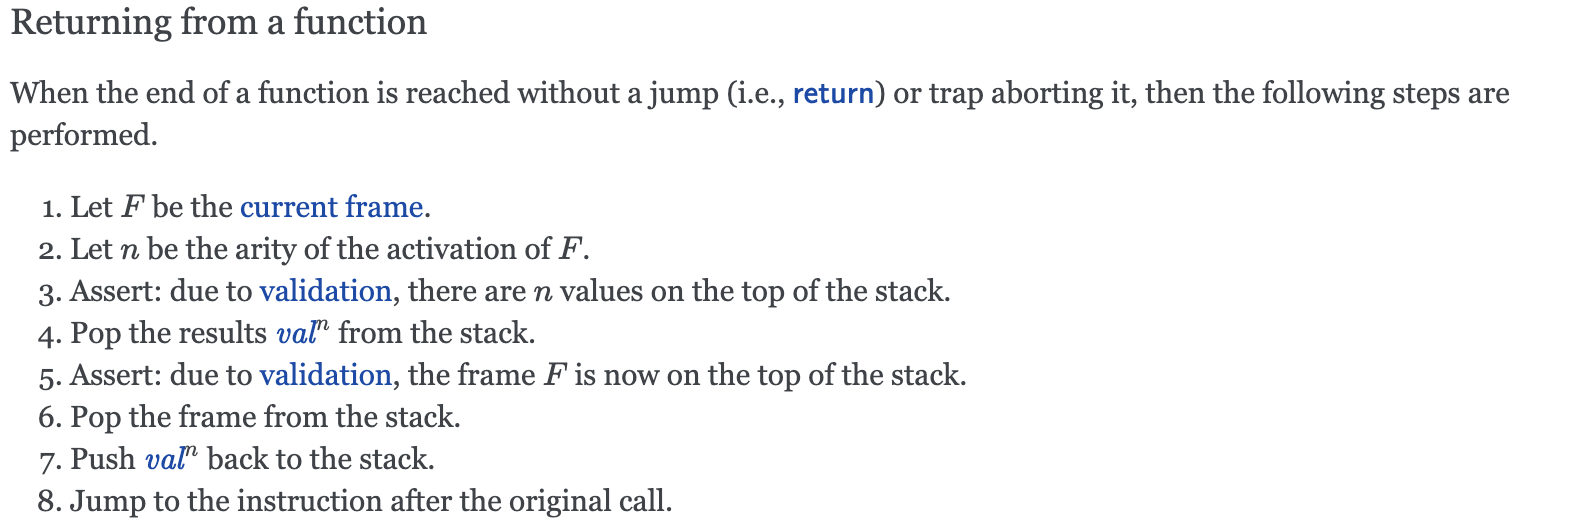
\includegraphics[width=15cm]{fig/returning}}
    \caption[Enter the caption title here]{returning from a function} \label{fig:returning}
\end{figure}

\section{Control flow in SpecTec prose}

% control flow structure in SpecTec prose
However, the \spectecp{} assumes a different model to explain the control flow
of WebAssembly.
Rather than using the notion of a pc, \spectecp{} assumes that WebAssembly
instructions are just given one by one.
This is because the \spectecp{} is generated automatically from the
\red{SpecTec DSL}.
\red{SpecTec DSL} uses rewrite rule to describe WebAssembly semantics, and it
is interpreted in \spectecp{} as consuming a WebAssembly instruction, pushing
or poping a control structures, and inputing new WebAssembly instructions.
It can be expressed in the following form:
$c^* \vdash i_0, i_1, ..., i_m \leadsto c'^* \vdash i'_0, ...i'_{m'}, i_1, ..., i_m$.
It means that given a sequence of contexts $c^*$, executing $i_0$ results in a
new sequence of contexts $c'^*$ and instructions $i'_0, ...i'_{m'}$.
To simply model the control flow of WebAssembly, other things not closely
related to the control flow are omitted in this notation.


% challenges in SpecTec prose
However, this viewpoint is challenged by the exiting label.
As the block structure doesn't remain intact in this model, it is hard to
describe \textbf{the end of the block}.
Furthermore, the exiting label is not performed by a specific WebAssembly
instruction, which makes it hard to model the behavior.
To handle this problem, an administrative instruction \texttt{end} is
introduced in \spectecp.
When entering a block, an \texttt{end} is appended to the end of the block.


% an example of Wasm control flow in official prose
\begin{figure}[h!]
    \centerline{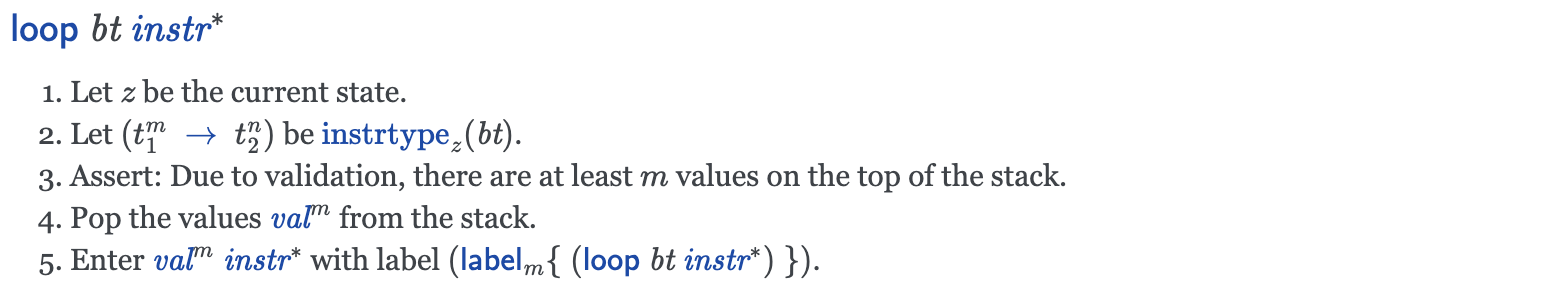
\includegraphics[width=15cm]{fig/spectec-loop}}
    \caption[Enter the caption title here]{SpecTec \texttt{loop}} \label{fig:spectec-loop}
\end{figure}
\begin{figure}[h!]
    \centerline{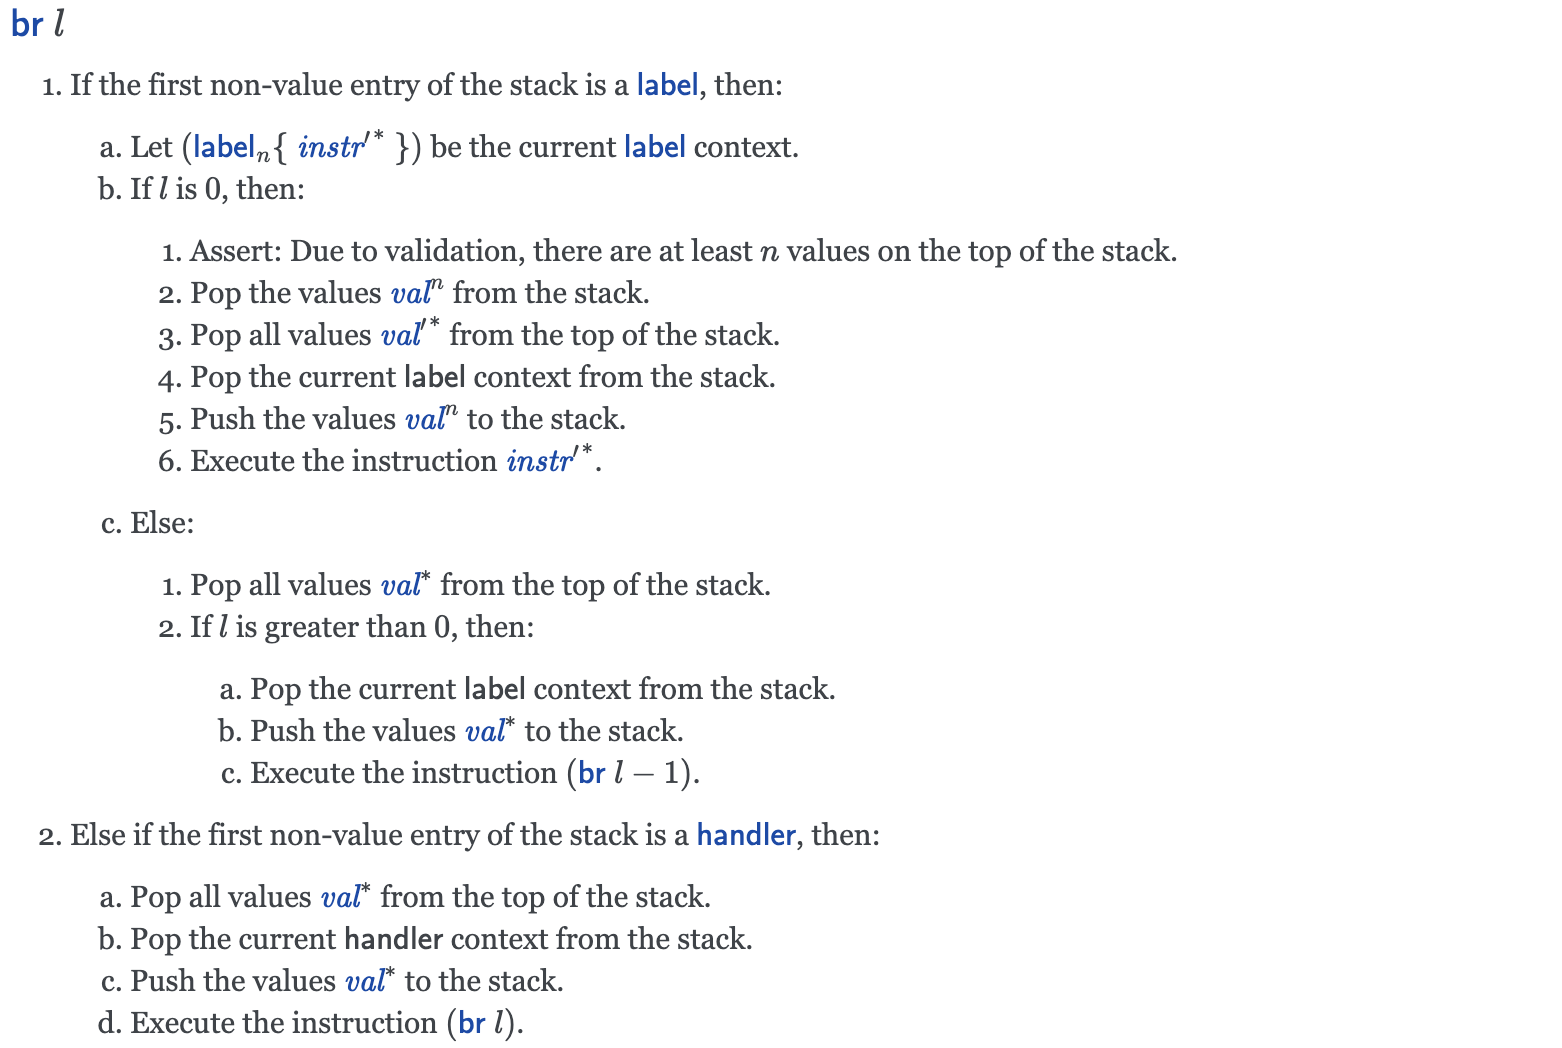
\includegraphics[width=15cm]{fig/spectec-br}}
    \caption[Enter the caption title here]{SpecTec \texttt{br}} \label{fig:spectec-br}
\end{figure}

\begin{align}
  &c^*
  \vdash
  loop([ ~ i32.const ~ 42, ~ br ~ 0, ~ unreachable ~ ]), ~ unreachable
  \label{eq:loop-1} \\
&\leadsto
  label(loop([ ~ i32.const ~ 42; ~ br ~ 0; ~ unreachable ~ ])), c^*
  \vdash
  i32.const ~ 42, ~ br ~ 0, ~ unreachable, ~ end, ~ unreachable
  \label{eq:loop-2} \\
  &\leadsto
  label(loop([ ~ i32.const ~ 42; ~ br ~ 0; ~ unreachable ~ ])), c^*
  \vdash
  ~ br ~ 0, ~ unreachable, ~ end, ~ unreachable
  \label{eq:loop-3} \\
&\leadsto
  c^*
  \vdash
  loop([ ~ i32.const ~ 42; ~ br ~ 0; ~ unreachable ~ ]), unreachable
  \label{eq:loop-4}
\end{align}

Consider example 1 above.
If we assume some control structure $c^*$ is given, the code can be expressed
like \cref{eq:loop-1}.
\cref{fig:spectec-loop} is the \spectecp{} of the \texttt{loop} instruction.
Rather than storing the point to jump as a continuation in the label, it stores
the \texttt{loop} instruction itself and \textit{enters} the block.
Here, \textit{enter} means that it pushes the label in the stack and executes
the instructions in the block, which means that \texttt{i32.const},
\texttt{br}, \texttt{unreachable}, \texttt{end} and \texttt{unreachable} become
the new inputs in \cref{eq:loop-2}.
When \texttt{i32.const} is excuted, it pushes 42 as \officialp{} does
in \cref{eq:loop-3}.
The value is omitted for brevity.
However, \texttt{br} behaves a bit differently.
\cref{fig:spectec-br} is the \spectecp{} of the \texttt{br} instruction.
It pops the label from the stack, removes the input instructions until the end
of the block, considers the loop instruction in the label as a new input
instruction.
Consequently, remaining inputs are \texttt{loop}, and \texttt{unreachable}
again in \cref{eq:loop-4}.
Therefore, it explains the same behavior in a different point of view.

\red{TODO: Also use example 3 to explain function call in official prose}

% an example of function call in official prose
\textbf{Example 3}
\begin{verbatim}
  // function definition of $push42
  (func $push42 (result i32) (i32.const 42))

  // function call
  (call $push42) (f32.const 3.14)
\end{verbatim}

\begin{align}
  &c^* \vdash call(\$push42), ~ f32.const ~ 3.14 \label{eq:call-1} \\
&\leadsto
  Label(\epsilon), ~ Frame(), ~ c^* \vdash i32.const ~ 42, ~ end, ~ f32.const ~ 3.14 \label{eq:call-2} \\
&\leadsto
  Label(\epsilon), ~ Frame(), ~ c^* \vdash end, ~ f32.const ~ 3.14 \label{eq:call-3} \\
&\leadsto
  c^* \vdash f32.const ~ 3.14 \label{eq:call-4} \\
&\leadsto
  c^* \label{eq:call-5}
\end{align}

Example 3 contains a function definition whose body is \texttt{i32.const}, a
\texttt{call} instruction followed by a \texttt{f32.const} instruction, which
can be expressed in \cref{eq:call-1}.
By invoking a function, it enters the block in \cref{eq:call-2}.
After executing the body in \cref{eq:call-3}, an \texttt{end} is executed.
In this point, this \texttt{end} represent both the end of the block and the
function.
As a consequence, this \text{end} perform both exiting label and returning from
a function in \cref{eq:call-4}, and the instruction after the \texttt{call} is
executed in \cref{eq:call-5}
It results in the values 42 and 3.14 pushed to the stack.


% summary & test
In short, the behavior of an \texttt{end} instruction 1) performs exiting
label, 2) looks up the top of the context, and 3) performs returing from a
function, if it is a frame.
The \spectecp{} can model the WebAssembly control flow using this \texttt{end}
instruction.
To show the correctness of the \spectecp{}, we run the WebAssembly tests
including official WebAssembly test suite by executing the \spectecp{} with
\red{definitional interpreter}.


% Problem
However, tests related to the control instruction are failed.
At that time, there was no explicit model to describe the control flow in
\spectecp{}, it was hard to define the problem, making it complicated to fix
the problem.





% official spec prose notation control structure
% seems to be pc-based
% AL from DSL ~ formal notation: no pc
% AL: instruction sequence input continously
% device exiting semantics for AL
% Executable spec passes all wasm testcases
% weird, maybe not happened in realworld, but valid wasm code
% wrong!
